% Options for packages loaded elsewhere
\PassOptionsToPackage{unicode}{hyperref}
\PassOptionsToPackage{hyphens}{url}
%
\documentclass[
]{article}
\title{DA3\_HW2\_Summary-Report}
\author{Gyebnar Daniel}
\date{2022 02 09}

\usepackage{amsmath,amssymb}
\usepackage{lmodern}
\usepackage{iftex}
\ifPDFTeX
  \usepackage[T1]{fontenc}
  \usepackage[utf8]{inputenc}
  \usepackage{textcomp} % provide euro and other symbols
\else % if luatex or xetex
  \usepackage{unicode-math}
  \defaultfontfeatures{Scale=MatchLowercase}
  \defaultfontfeatures[\rmfamily]{Ligatures=TeX,Scale=1}
\fi
% Use upquote if available, for straight quotes in verbatim environments
\IfFileExists{upquote.sty}{\usepackage{upquote}}{}
\IfFileExists{microtype.sty}{% use microtype if available
  \usepackage[]{microtype}
  \UseMicrotypeSet[protrusion]{basicmath} % disable protrusion for tt fonts
}{}
\makeatletter
\@ifundefined{KOMAClassName}{% if non-KOMA class
  \IfFileExists{parskip.sty}{%
    \usepackage{parskip}
  }{% else
    \setlength{\parindent}{0pt}
    \setlength{\parskip}{6pt plus 2pt minus 1pt}}
}{% if KOMA class
  \KOMAoptions{parskip=half}}
\makeatother
\usepackage{xcolor}
\IfFileExists{xurl.sty}{\usepackage{xurl}}{} % add URL line breaks if available
\IfFileExists{bookmark.sty}{\usepackage{bookmark}}{\usepackage{hyperref}}
\hypersetup{
  pdftitle={DA3\_HW2\_Summary-Report},
  pdfauthor={Gyebnar Daniel},
  hidelinks,
  pdfcreator={LaTeX via pandoc}}
\urlstyle{same} % disable monospaced font for URLs
\usepackage[margin=1in]{geometry}
\usepackage{graphicx}
\makeatletter
\def\maxwidth{\ifdim\Gin@nat@width>\linewidth\linewidth\else\Gin@nat@width\fi}
\def\maxheight{\ifdim\Gin@nat@height>\textheight\textheight\else\Gin@nat@height\fi}
\makeatother
% Scale images if necessary, so that they will not overflow the page
% margins by default, and it is still possible to overwrite the defaults
% using explicit options in \includegraphics[width, height, ...]{}
\setkeys{Gin}{width=\maxwidth,height=\maxheight,keepaspectratio}
% Set default figure placement to htbp
\makeatletter
\def\fps@figure{htbp}
\makeatother
\setlength{\emergencystretch}{3em} % prevent overfull lines
\providecommand{\tightlist}{%
  \setlength{\itemsep}{0pt}\setlength{\parskip}{0pt}}
\setcounter{secnumdepth}{-\maxdimen} % remove section numbering
\usepackage{booktabs}
\usepackage{longtable}
\usepackage{array}
\usepackage{multirow}
\usepackage{wrapfig}
\usepackage{float}
\usepackage{colortbl}
\usepackage{pdflscape}
\usepackage{tabu}
\usepackage{threeparttable}
\usepackage{threeparttablex}
\usepackage[normalem]{ulem}
\usepackage{makecell}
\usepackage{xcolor}
\usepackage{siunitx}
\newcolumntype{d}{S[input-symbols = ()]}
\ifLuaTeX
  \usepackage{selnolig}  % disable illegal ligatures
\fi

\begin{document}
\maketitle

\hypertarget{assessment-of-rbnb-aparment-prices-in-rome}{%
\section{Assessment of rbnb aparment prices in
Rome}\label{assessment-of-rbnb-aparment-prices-in-rome}}

\hypertarget{goal-and-data-used}{%
\subsection{Goal and data used}\label{goal-and-data-used}}

CityRent, a company specialized in operating rbnb apartments in major
European cities, aims to enter the market in Rome.

The goal of this paper is to summaries the key findings regarding the
pricing mechanism of small and mid sized rbrb apartments in Rome. The
paper will give insights on the market, how to best price the apartments
given its key attributes, and what the best practices are for operating
these apartments.

The study was conducted using data from
\url{http://insideairbnb.com/get-the-data.html}. The models were built
on a data set containing 16.273 observations and 416 variables.

\hypertarget{market-overview}{%
\subsection{Market overview}\label{market-overview}}

The rbnb market in Rome is concetrated in district I with 52\% of
selected listings being located there with a median price of EUR 86,
which is significantly higher than in other districts.

\begin{table}
\centering
\begin{tabular}[t]{llrrrrr}
\toprule
neighbourhood\_cleansed &   & N & Percent & Mean & Median & SD\\
\midrule
I Centro Storico & price & 8778 & \num{54.12} & \num{98.80} & \num{86.00} & \num{52.61}\\
II Parioli/Nomentano & price & 1130 & \num{6.97} & \num{76.20} & \num{65.00} & \num{46.68}\\
III Monte Sacro & price & 250 & \num{1.54} & \num{60.35} & \num{53.50} & \num{32.76}\\
IV Tiburtina & price & 302 & \num{1.86} & \num{58.72} & \num{50.00} & \num{42.61}\\
IX Eur & price & 188 & \num{1.16} & \num{70.51} & \num{63.00} & \num{39.40}\\
V Prenestino/Centocelle & price & 670 & \num{4.13} & \num{50.72} & \num{46.00} & \num{24.70}\\
VI Roma delle Torri & price & 116 & \num{0.72} & \num{57.02} & \num{49.00} & \num{35.82}\\
VII San Giovanni/CinecittĂ  & price & 1193 & \num{7.36} & \num{66.51} & \num{60.00} & \num{35.74}\\
VIII Appia Antica & price & 493 & \num{3.04} & \num{68.13} & \num{60.00} & \num{39.00}\\
X Ostia/Acilia & price & 405 & \num{2.50} & \num{76.46} & \num{61.00} & \num{46.11}\\
XI Arvalia/Portuense & price & 294 & \num{1.81} & \num{62.74} & \num{59.00} & \num{29.83}\\
XII Monte Verde & price & 848 & \num{5.23} & \num{73.03} & \num{66.00} & \num{37.24}\\
XIII Aurelia & price & 975 & \num{6.01} & \num{76.74} & \num{69.00} & \num{39.86}\\
XIV Monte Mario & price & 339 & \num{2.09} & \num{69.61} & \num{60.00} & \num{41.93}\\
XV Cassia/Flaminia & price & 238 & \num{1.47} & \num{73.83} & \num{60.00} & \num{43.66}\\
\bottomrule
\end{tabular}
\end{table}

\hypertarget{key-decision-points}{%
\subsection{Key decision points}\label{key-decision-points}}

\hypertarget{observation-selection}{%
\paragraph{Observation selection}\label{observation-selection}}

I excluded apartments above 400 EUR per night. This cutoff still leaves
plenty of extreme values as the 3rd quartile is 100 EUR. I dropped
observations where price was missing (see histogram of prices below)

\hypertarget{variable-selection}{%
\paragraph{Variable selection}\label{variable-selection}}

I selected 40 variables from the original data set (apart from
amenities). I excluded variables that were redundant, had very little
variation, or variables with irrelevant underlying meaning based on my
domain knowledge.

\hypertarget{dealing-with-nas}{%
\paragraph{Dealing with NAs}\label{dealing-with-nas}}

Variables regarding the reviews had many, c.20\% missing values. I
flagged these missing values and imputed 0 in order to keep the
variables numeric. Variables regarding the host (eg. host since,
superhost, ect.) had only a few missing values (\textless5\%) so I
decided to impute them with the median. For the few missing integer
values, I imputed a replacement value from another variable based on
domain knowledge (e.g.~missing number of beds equal to number of
accommodates, missing number of bedrooms equal to accommodates divided
by 2)

\hypertarget{feature-engineering}{%
\paragraph{Feature engineering}\label{feature-engineering}}

I clustered variables into factors, dummies and numeric. For a
categorical variable with many values I created a factor,
e.g.~Neighborhood, for categorical with 2 values I created a dummy with
0 or 1, and for numeric integers I decided individually whether to keep
as numeric or to transform to factors (e.g.~accommodates). I also
created two additional variables, bathroom-bedroom ratio, and host years
of experience.

\hypertarget{amenities}{%
\paragraph{Amenities}\label{amenities}}

I extracted all 379 amenities from the raw data, organized it into a
dataframe, ordered it according to frequency, and included it into the
model as separate dummy variables (e.g.~is there a TV)

\hypertarget{key-findings-and-reccomendations}{%
\subsection{Key findings and
reccomendations}\label{key-findings-and-reccomendations}}

\hypertarget{market-insights}{%
\paragraph{Market insights}\label{market-insights}}

The histogram of price per night suggest that the typical apartment
costs EUR 74 per night, and the average is EUR 85.

\begin{figure}

{\centering 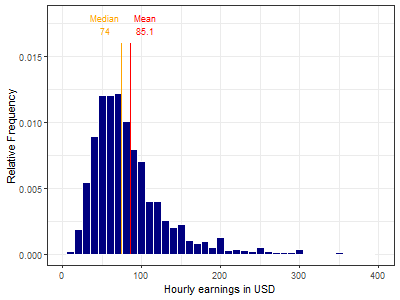
\includegraphics[width=0.5\linewidth]{https://raw.githubusercontent.com/DaniDataScience/DA_3/main/DA3/Assignment_2/plot_price_hist} 

}

\caption{Histogram of prices per night}\label{fig:unnamed-chunk-2}
\end{figure}

\hypertarget{key-attributes-to-consider}{%
\paragraph{Key attributes to
consider}\label{key-attributes-to-consider}}

The variables that are the most important are reviews regarding the
location, the total listings of hosts (suggesting that professionals
with more listings have higher prices), number of accommodates, and the
ratio of bathrooms to guests (based on variable importance plots from
annex).

We also look in detail at amenities, and the most important ones are the
dishwasher, the AC, free parking, and having an elevator.

Looking at the importance of feature groups, the features that describe
the quality of the host are the most imporant. Meaning that operating
the appartments are jsut as important. The attributes describing the
location are jsut second to the ones describing the host!

\hypertarget{apparment-location-and-size}{%
\paragraph{Apparment location and
size}\label{apparment-location-and-size}}

In order to be able to charge a highest possible price, CityRent should
aim to purchase an apartment in the most popular district I, where c
40\% of selected listings are to be found. However, district II, XIV,
XII is also a potentially good target, as the price per night might be
lower but the investment cost to purchase an apartment could be even
more lower - this question should be evaluated in the next steps.

Such an apartment would have a price of xx per night which is above the
average of xx and the median of xx

\hypertarget{modeling-process}{%
\subsection{Modeling process}\label{modeling-process}}

I have grouped the variables into five categories, based on what they
represent:

\begin{itemize}
\tightlist
\item
  property: contains variables that describe the location and the type
  of real estate, e.g.~neighborhood, property type
\item
  size: contains variables that describe the size of the real estate and
  its layout, e.g.: beds, bathrooms, number of accommodations,
  bathroom-guest ratio
\item
  host: contains variables that describe the details about the host,
  e.g.~is the host a local, how many years of experience the host has
\item
  booking: contains variables that describe the booking options,
  e.g.~minimum nights, response time
\item
  reviews: contains variables on the reviews, e.g.~overall rating,
  number of reviews, and the flags of missing values
\item
  amenities: contains items and extras that are available, e.g.~TV, AC,
  ect. I created 3 variations to this group, to be used as model
  complexity increases: one with 10 and one with 50 most frequent
  amenity, and one with all 379 amenities (amenities 2, 3, and 4)
\item
  interactions: I created interactions, mostly for the number of guests,
  reviews, and neighborhood, and their combination
\end{itemize}

I have created the following formulas, with model 1 being the simplest,
and model 4 being a reasonably complex model with top 50 amenities, and
model 5 with all 379 amenities:

\begin{itemize}
\tightlist
\item
  model 1: simplest model with n\_accommodates as the only variable
\item
  model 2: price \textasciitilde{} size, property
\item
  model 3: price \textasciitilde{} size, property, reviews, amenities\_2
\item
  model 4: price \textasciitilde{} size, property, reviews, host,
  booking, amenities\_3, interactions
\item
  model 5: price \textasciitilde{} size, property, reviews, host,
  booking, amenities\_4, interactions
\end{itemize}

From model 1-5 I created OLS models with 5-fold cross validation, and
selected model 4 for Random Forest and GBM. I used the most complex
model, model 5, for LASSO.

After training, I evaluated the OLS, the LASSO, the Random Forest, and
the GBM model on the holdout set.

I used the coefficients of the OLS model to explain the key insights on
the market in general, and I used the partial dependence plot of the GBM
and the variable importance plot from the Random Forest to draw my
conclusions.

\hypertarget{interpretation-of-model-results}{%
\subsection{Interpretation of model
results}\label{interpretation-of-model-results}}

The initial 5 models with OLS performed as expected: - Model 4 gave the
best result, due to having the lowest RMSE and only a slighter higher
BIC than the less complex Model 3, which performed with a much higher
RMSE (by EUR 0.8) - Model 5 is overfit, and was thus used with LASSO.
This resulted in a very slightly lower RMSE than the best OLS model, OLS
M4 (43.03 EUR vs 43.07 EUR) - Regarding the number of coefficients,
LASSO excluded 158 variables from the 380

\begin{table}

\caption{\label{tab:unnamed-chunk-3}OLS and LASSO detailed results}
\centering
\begin{tabular}[t]{l|r|r|r|r|r}
\hline
Model & Coefficients & R\_squared & BIC & Training\_RMSE & Test\_RMSE\\
\hline
OLS M1 & 2 & 0.1259401 & 138642.4 & 49.64776 & 49.63445\\
\hline
OLS M2 & 31 & 0.2627405 & 136701.2 & 45.59731 & 45.70278\\
\hline
OLS M3 & 57 & 0.3237695 & 135822.7 & 43.66932 & 43.91519\\
\hline
OLS M4 & 129 & 0.3561310 & 135866.4 & 42.61160 & 43.06855\\
\hline
OLS M5 & 380 & 0.3812255 & 137726.8 & 41.77296 & 43.14609\\
\hline
LASSO M5 & 212 & 0.3436237 & NA & NA & 43.02903\\
\hline
\end{tabular}
\end{table}

The graph below shows how test RMSE decreases until Model 4, while
increases for Model 5

\begin{figure}

{\centering 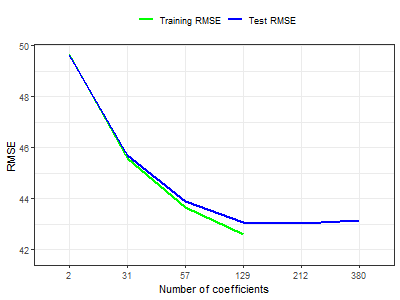
\includegraphics[width=0.5\linewidth]{https://raw.githubusercontent.com/DaniDataScience/DA_3/main/DA3/Assignment_2/plot_trainings_vs_test_rmse} 

}

\caption{Test & Train RMSE by coefficients for OLS models}\label{fig:unnamed-chunk-4}
\end{figure}

My conclusion is that the well constructed Model 4 performed only
slightly below the LASSO model. I selected to use Model 4 for another
roudn of calculations with Random Forest and GBM

Based on the OLS for model 1-5, model 4 is the optimal model, as it has
the lowest RMSE on the test set, and its BIC is not significantly higher
than for model 3, a less complex model with a higher RMSE - Model 5
clearly overfits the data, given that the train RMSE is lower but the
test RMSE is higher compared to model 5.

\begin{table}

\caption{\label{tab:unnamed-chunk-5}RMSE on the holdout set}
\centering
\begin{tabular}[t]{l|r|r}
\hline
Model & CV.RMSE & Holdout.RMSE\\
\hline
OLS M4 & 43.11349 & 42.63775\\
\hline
LASSO M5 & 43.02903 & 42.42538\\
\hline
RF M4 & 43.02483 & 42.59012\\
\hline
GBM M4 & 42.34146 & 41.79039\\
\hline
\end{tabular}
\end{table}

The RMSE on the holdout sample is slightly below than the RMSE for the
coros-validated test set. The lowest RMSE is for Model 4 with GBM
method, followed by the LASSO on Model 5, and Random Forest and OLS on
Model 4

\hypertarget{annex}{%
\subsection{Annex}\label{annex}}

\hypertarget{pdp-plots}{%
\paragraph{PDP Plots}\label{pdp-plots}}

\begin{figure}

{\centering 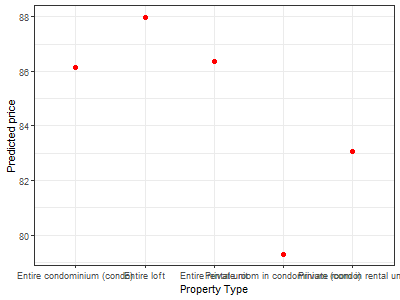
\includegraphics[width=0.5\linewidth]{https://raw.githubusercontent.com/DaniDataScience/DA_3/main/DA3/Assignment_2/plot_pdp_property} 

}

\caption{PDP by property type}\label{fig:unnamed-chunk-6}
\end{figure}

\begin{figure}

{\centering 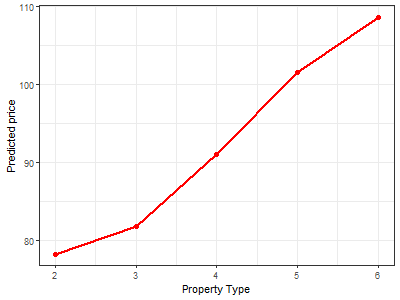
\includegraphics[width=0.5\linewidth]{https://raw.githubusercontent.com/DaniDataScience/DA_3/main/DA3/Assignment_2/plot_pdp_n_accommodates} 

}

\caption{PDP by number of accomodates}\label{fig:unnamed-chunk-7}
\end{figure}

\begin{figure}

{\centering 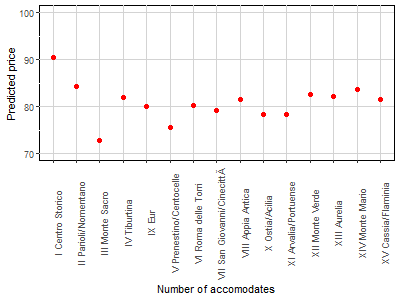
\includegraphics[width=0.5\linewidth]{https://raw.githubusercontent.com/DaniDataScience/DA_3/main/DA3/Assignment_2/plot_pdp_f_neighbourhood_cleansed} 

}

\caption{PDP by neighborhood}\label{fig:unnamed-chunk-8}
\end{figure}

\hypertarget{variable-importance-plots}{%
\paragraph{Variable importance plots}\label{variable-importance-plots}}

\begin{figure}

{\centering 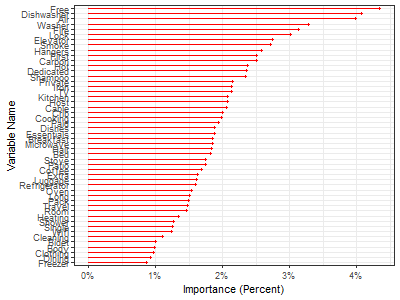
\includegraphics[width=0.5\linewidth]{https://raw.githubusercontent.com/DaniDataScience/DA_3/main/DA3/Assignment_2/imp_grouped} 

}

\caption{Variable importance by feature groups}\label{fig:unnamed-chunk-9}
\end{figure}

\begin{figure}

{\centering 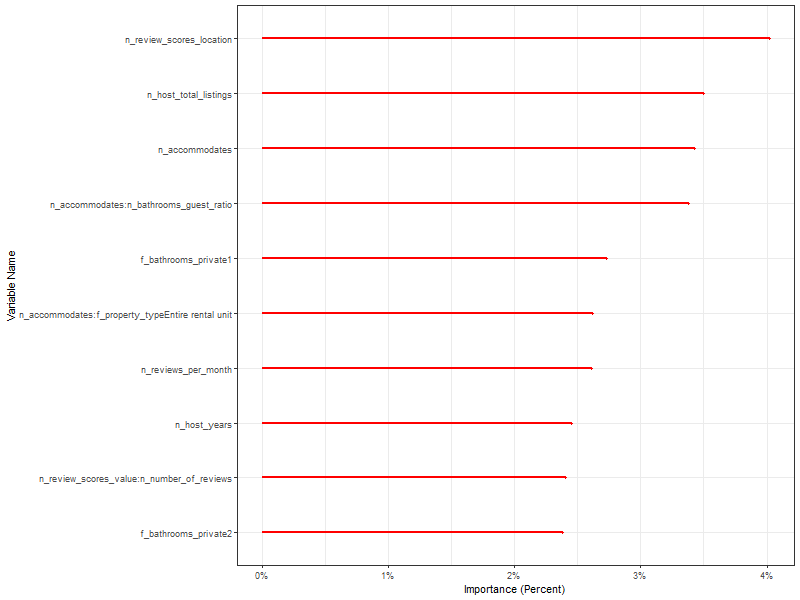
\includegraphics[width=0.5\linewidth,height=2\textheight]{https://raw.githubusercontent.com/DaniDataScience/DA_3/main/DA3/Assignment_2/imp_top10} 

}

\caption{Variable importance of top 10 variables}\label{fig:unnamed-chunk-10}
\end{figure}

\begin{figure}

{\centering 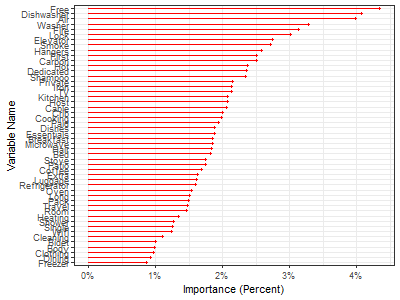
\includegraphics[width=0.5\linewidth]{https://raw.githubusercontent.com/DaniDataScience/DA_3/main/DA3/Assignment_2/imp_amen} 

}

\caption{Variable importance of amenities}\label{fig:unnamed-chunk-11}
\end{figure}

\end{document}
